% !TEX root = ../main.tex
\chapter{Nonlinear Spectroscopy and Two-Dimensional Electronic Spectra}
\label{chapter_spectroscopy}

%------------------------------------------------------------------------------
% 0. Motivation and Historical Development
%------------------------------------------------------------------------------

\section{Motivation and Historical Development}
\label{sec:spectroscopy_motivation}
Spectroscopy studies how matter interacts with energy, most commonly through absorption, emission, or scattering of radiation~\cite{skoogetal2017principlesinstrumentalanalysis}.
Because atoms and molecules occupy discrete energy levels, optical transitions satisfy the Planck relation $\Delta E=h\nu=hc/\lambda$.
Early spectroscopy exploited this to identify characteristic line spectra that served as fingerprints of quantized structure~\cite{balmer1885notizuberspectrallinien, rydberg1890xxxivstructurelinespectra, bohr1913constitutionatomsmolecules}.
Quantum mechanics later connected these lines to transitions between eigenstates of the microscopic Hamiltonian~\cite{berman2011principleslaserspectroscopy, dirac1927quantumtheoryemission}.
In practice, transitions are often labelled by the wavenumber $\tilde{\nu}=1/\lambda\;[\mathrm{cm}^{-1}]$, which is proportional to the transition energy.
The electronic transitions studied in this thesis lie in the visible and near-UV range, $\tilde{\nu}\sim 13\,000$--$25\,000\,\mathrm{cm}^{-1}$, where coherence and relaxation dynamics unfold on femtosecond timescales.

For decades, spectroscopy was essentially linear: a weak field probes the sample and one records intensity as a function of frequency.
Linear absorption and emission reveal excitation energies, oscillator strengths, and broadening mechanisms, such as natural linewidth or Doppler broadening~\cite{skoogetal2017principlesinstrumentalanalysis}.
However, a one-dimensional line shape compresses distinct dynamical processes---coherence loss, population transfer, and environment-induced frequency fluctuations---into a single spectral profile.
This makes different microscopic mechanisms difficult to disentangle.

The induced polarisation $\boldsymbol{P}(t)$ contains not only components linear in the applied field $\boldsymbol{E}(t)$~\cite{kubo1957statisticalmechanicaltheoryirreversible},
\begin{equation*}
\boldsymbol{P}^{(1)}(t) = \int_{0}^{\infty}\!\mathrm{d}\tau\;
\boldsymbol{R}^{(1)}(\tau)\!\cdot\!\boldsymbol{E}(t-\tau),
\end{equation*}
where $\boldsymbol{R}^{(1)}$ is the causal linear-response kernel.
There are also quadratic, cubic, and higher-order contributions,
\begin{equation*}
	\boldsymbol{P}^{(n)}(t) \propto \boldsymbol{E}(t)^n,\qquad n\ge 2.
\end{equation*}

These terms generate effects such as second-harmonic generation, four-wave mixing, and stimulated Raman scattering.
Conceptually, they probe multi-time correlation functions of the system.
Therefore, they encode dynamical information that is inaccessible in the linear regime~\cite{frankenetal1961generationopticalharmonics, mukamel1995principlesnonlinearoptical}.

Two-dimensional Fourier-transform spectroscopy is a powerful tool within nonlinear spectroscopy.
By correlating excitation and detection frequencies, it separates homogeneous from inhomogeneous broadening.
Homogeneous broadening reflects the intrinsic linewidth of a single chromophore, set by coherence loss and population relaxation.
Inhomogeneous broadening, by contrast, arises from static disorder in the molecular environment (e.g.\ different binding sites or solvent configurations), which distributes transition frequencies across the ensemble.
This separation allows the homogeneous linewidth to be extracted even in strongly inhomogeneously broadened systems~\cite{bangertetal2022highresolutiontwodimensionalelectronic, freschetal2023twodimensionalelectronicspectroscopy}.
In addition, two-dimensional spectra track spectral diffusion---time-dependent fluctuations of transition frequencies caused by a slowly evolving local environment---through the loss of frequency--frequency correlation with waiting time~\cite{cho2009twodimensionalopticalspectroscopy,mukamel1995principlesnonlinearoptical}.
Cross peaks further visualize couplings between transitions and energy-transfer pathways, which are central to the analyses in this thesis.

To connect these experimental capabilities to the theoretical framework developed in~\autoref{chapter_open_quantum_systems}, this thesis uses the response-function formalism.
It links a given pulse sequence to the measured signal via the induced polarisation.
By separating matter and field contributions, this formalism makes the perturbative order explicit.
The matter-side derivation---how incident fields generate $\boldsymbol{P}^{(n)}$---is given in~\autoref{app:response_functions} and shows how open-system master equations, such as the Redfield equation (microscopically derived in~\autoref{sec:Redfield_eq}), enter spectroscopy.
The field-side derivation---how $\boldsymbol{P}^{(3)}$ radiates the signal---is given in~\autoref{app:2dfts_maxwell}.

The remainder of this chapter is organized as follows.
\autoref{sec:light_matter} introduces the semiclassical light--matter Hamiltonian in the dipole approximation, which establishes the fundamental microscopic interaction governing how laser pulses perturb molecular systems and provides the starting point for all spectroscopic calculations in this thesis.
\autoref{sec:pol_and_macr_response} provides a unified summary of the two technical appendices by combining the matter-side response expansion with the Maxwell-side radiation step into one signal chain.
\autoref{sec:response_formalism} then states the core response-function expressions and pathway structure used in the spectroscopy workflow.
Finally, \autoref{sec:three_pulse_geometry}--\autoref{sec:2D_construction_formal} applies these ingredients to three-pulse experiments, phase matching, phase cycling, and 2D spectrum construction.

%------------------------------------------------------------------------------
% 2. Light--Matter Interaction and Semiclassical Hamiltonian
%------------------------------------------------------------------------------
\section{Light--Matter Interaction}
\label{sec:light_matter}
Throughout this thesis, the electromagnetic field is treated as a classical, time-dependent drive, while the matter degrees of freedom are described quantum mechanically.
The central object is the density matrix of the matter, whose evolution determines the optical response.

The microscopic dynamics of the full system (molecule plus environment) are governed by the Liouville--von Neumann equation (cf.~\autoref{eq:Von_Neumann_Equation})
\begin{equation}
	\frac{d}{dt}\hat{\rho}_{\mathrm{T}}(t) = -i\,[\hat{H}(t),\hat{\rho}_{\mathrm{T}}(t)],
	\label{eq:LvN_total_spectroscopy}
\end{equation}
with total Hamiltonian
\begin{equation*}
	\hat{H}(t)=\hat{H}_{\mathrm{S}}(t)+\hat{H}_{\mathrm{E}}+\hat{H}_{\mathrm{int}}.
\end{equation*}
Here $\hat{H}_{\mathrm{E}}$ is the environment Hamiltonian and $\hat{H}_{\mathrm{int}}$ the system--environment coupling.
The semiclassical light field enters only through the time-dependent system Hamiltonian $\hat{H}_{\mathrm{S}}(t)$.
The structure therefore is a time-dependent version of the one used in~\autoref{sec:setup_system_environment}.

\subsection{Minimal Coupling}
\label{subsec:minimal_coupling}

Mathematical details can be found in~\cite{cohen-tannoudjietal2008atomphotoninteractionsbasic,berman2011principleslaserspectroscopy}.
In Coulomb gauge, the interaction of a particle of mass $m$ and charge $q$ with a classical electromagnetic field is described by the minimal-coupling Hamiltonian
\begin{equation*}
	\hat{H}(\hat{\boldsymbol{r}}, t)
	= \frac{1}{2m}\Bigl[\hat{\boldsymbol{p}} + q\,\boldsymbol{A}(\hat{\boldsymbol{r}},t)\Bigr]^2
	+ V(\hat{\boldsymbol{r}}) - q\,\phi(\hat{\boldsymbol{r}},t),
\end{equation*}
where $\boldsymbol{A}$ and $\phi$ are the vector and scalar potentials of the external field, $V$ is the static binding potential, $\boldsymbol{p}$ is the canonical momentum operator, and $\hat{\boldsymbol{r}}$ is the position operator.
The transverse electric field is related to the vector potential by
\begin{equation*}
	\boldsymbol{E}_\perp(\boldsymbol{r},t)=-\frac{\partial \boldsymbol{A}(\boldsymbol{r},t)}{\partial t}.
\end{equation*}

In most optical settings the wavelength is much larger than the molecular size, so the field varies negligibly across the system.
In this limit, a unitary transformation leads to an equivalent effective Hamiltonian
\begin{equation*}
	\hat{H}_{\mathrm{S}}(t)=\hat{H}_0 - \hat{\boldsymbol{\mu}}\cdot\boldsymbol{E}(t),
\end{equation*}
with $\hat{H}_0$ the field-free Hamiltonian and $\hat{\boldsymbol{\mu}}=-q\,\hat{\boldsymbol{r}}$ the electric dipole operator.
For a fixed linear polarisation direction $\boldsymbol{e}$, define
\begin{equation*}
	E(t)=\boldsymbol{e}\cdot\boldsymbol{E}(t),
	\qquad
	\hat{\mu}=\hat{\boldsymbol{\mu}}\cdot\boldsymbol{e},
\end{equation*}
so that
\begin{equation*}
	\hat{H}_{\mathrm{S}}(t)=\hat{H}_0 - \hat{\mu}\,E(t).
\end{equation*}

A key simplification used throughout is the rotating-wave approximation (RWA).
It is introduced here and defined again in~\autoref{eq:E_plusminus}; its role in pathway selection is discussed in~\autoref{subsec:rephasing_nonrephasing}.
For narrow-linewidth transitions driven near resonance, the field is decomposed into positive- and negative-frequency components $\boldsymbol{E}^{(+)}$ and $\boldsymbol{E}^{(-)}$, and only the near-resonant cross terms $\hat{\boldsymbol{\mu}}^{(+)}\!\cdot\!\boldsymbol{E}^{(-)}$ and $\hat{\boldsymbol{\mu}}^{(-)}\!\cdot\!\boldsymbol{E}^{(+)}$ remain in the equation of motion.

\section{Microscopic and Macroscopic Response}
\label{sec:pol_and_macr_response}
This section summarizes, in one place, the two complementary derivations developed in the appendices. The next sections then build on this summary to detail the response-function formalism and its application to 2D spectroscopy.

For a representative molecule, the microscopic polarisation is the expectation value of the electric dipole operator,
\begin{equation}
\boldsymbol{P}(t)
= \mathrm{Tr}_{\mathrm{S}}\!\bigl[
\hat{\boldsymbol{\mu}}\,\hat{\rho}_{\mathrm{S}}(t)
\bigr].
\label{eq:P_def_spectroscopy}
\end{equation}
Physically, $\boldsymbol{P}(t)$ quantifies the laser-driven redistribution of charge within the molecule.
The field induces charge displacements, and these microscopic motions are the origin of the polarisation that ultimately acts as a source for the emitted electromagnetic signal.
On a microscopic level, the polarisation density can be understood directly in terms of moving charges.
Consider charges $q_i$ at positions $\boldsymbol r_i(t)$:
\begin{equation*}
	\boldsymbol P(\boldsymbol r, t)
		\sim \sum_i q_i \boldsymbol r_i(t)\, \delta(\boldsymbol r - \boldsymbol r_i(t)).
\end{equation*}
The macroscopic polarisation field $\boldsymbol P(\boldsymbol r,t)$ is obtained by coarse-graining over a small volume.
This volume must be large compared to molecular dimensions, but small on macroscopic scales.
Appropriate averaging then yields the macroscopic quantity~\cite{mancal2022nonlinearopticalspectroscopy}.

Here $\hat{\rho}_{\mathrm{S}}(t)=\mathrm{Tr}_{\mathrm{E}}\,\hat{\rho}_{\mathrm{T}}(t)$ is obtained by tracing out the environment from the total state, and it follows the reduced open-system dynamics introduced in~\autoref{chapter_open_quantum_systems}.
In practice, dissipative effects like population relaxation and dephasing enter through this reduced evolution, which provides the dynamical input to the matter-side response derivation in~\autoref{app:response_functions}.

In the perturbative regime, the macroscopic polarisation is expanded as
\begin{equation*}
\boldsymbol{P}
=\boldsymbol{P}^{(1)}
+\boldsymbol{P}^{(3)}+\cdots.
\end{equation*}
The field-side derivation then yields the wave equation with polarisation source term,
\begin{equation*}
	\nabla \times \nabla \times \boldsymbol{E}(\boldsymbol{r}, t)
	+ \frac{1}{c^2} \frac{\partial^2}{\partial t^2}
	\boldsymbol{E}(\boldsymbol{r}, t)
	= - \mu_0 \frac{\partial^2}{\partial t^2}
	\boldsymbol{P}(\boldsymbol{r}, t).
\end{equation*}
In a four-wave-mixing experiment with heterodyne detection (see~\autoref{sec:detection_schemes}), the recorded quantity is linear in the emitted field and therefore in the selected third-order polarisation component,
\begin{equation*}
	\boldsymbol{E}_{\mathrm{S}}^{(3)}(\boldsymbol{r},t)
	\propto
	i\,\boldsymbol{P}^{(3)}(\boldsymbol{r},t).
\end{equation*}
This closes the link between microscopic dynamics and the measured signal: the material model determines $R^{(3)}$, $R^{(3)}$ determines $P^{(3)}$, and Maxwell propagation/detection map $P^{(3)}$ to the observable field.
The combined result of both appendices is the practical spectroscopy chain used throughout this thesis: the third-order response function $R^{(3)}$ determines the third-order polarisation $P^{(3)}$, which generates the emitted signal field $E_{\mathrm{S}}$, from which the detected signal $\tilde{E}_{\mathrm{S}}$ is obtained.
\autoref{sec:response_formalism} now details the first link, i.e.
the response-function construction of $R^{(3)}$ and its pathway decomposition.

\section{Response Function Formalism}
\label{sec:response_formalism}
The response-function formalism connects the applied field $\boldsymbol{E}(t)$ to the induced polarisation $\boldsymbol{P}^{(n)}(t)$.
%The full derivation is given in~\autoref{app:response_functions}. 
Here the key results are stated for linear response ($n=1$) and, most importantly for this thesis, for third-order response ($n=3$).

Linear response is the simplest setting in which the causal time-domain structure is explicit and the Liouville-space pathway structure first appears.
For these reasons, it is discussed in detail.

\subsection{Linear Response and the Kubo Formula}
\label{sec:linear_response}
Specialising~\autoref{eq:app_Pn_convolution_scalar} and~\autoref{eq:app_Sn_def_scalar} to $n=1$ gives
\begin{equation}
\boldsymbol{P}^{(1)}(t)
= \int_{0}^{\infty}\!\mathrm{d}\tau_1\,\boldsymbol{R}^{(1)}(\tau_1)\,E(t-\tau_1),
\label{eq:P1_convolution_thesis}
\end{equation}
with
\begin{equation}
\boldsymbol{R}^{(1)}(\tau_1)
= \mathrm{i}\,\mathrm{Tr}\bigl\{\hat{\boldsymbol{\mu}}\,\mathcal{U}_0(\tau_1)\,\mathcal{V}[\hat{\rho}_{\mathrm{eq}}]\bigr\}.
\label{eq:S1_def_superop_thesis}
\end{equation}

Even at first order, \autoref{eq:S1_def_superop_thesis} contains two Liouville-space pathways.
Expanding the commutator gives a difference of two time-ordered dipole correlation functions, which motivates defining
\begin{equation}
	J_{1}(\tau) \equiv \mathrm{Tr}\bigl\{\hat{\mu}_{\mathrm{I}}(\tau)\,\hat{\mu}_{\mathrm{I}}(0)\,\hat{\rho}_{\mathrm{eq}}\bigr\},
	\label{eq:J1_definitions}
\end{equation}
so that the causal response can be written as
\begin{equation}
	R^{(1)}(\tau) = i\,\Theta(\tau)\,\bigl[J_{1}(\tau)-J_{1}^*(\tau)\bigr].
	\label{eq:R1_J1_J1*}
\end{equation}
The two terms correspond to interactions on the ket and on the bra, with a relative minus sign.

To make this structure explicit, consider the simplest example of a two-level system.
This allows the general expressions to be evaluated in closed form and introduces the double-sided Feynman representation that will later be used for higher-order processes (see~\autoref{sec:third_order_response}).

\subsubsection{Two-Level System}
\label{sec:two_level_system_linear_response}
Consider a system with electronic states $\ket{g}$ and $\ket{e}$.
For optical transitions ($\omega_{eg}\sim \tilde{\nu}_0 \approx 16\,000\,\mathrm{cm}^{-1}$), the excited-state thermal population at room temperature is negligible.
Therefore, the initial condition can be approximated as the electronic ground state,
\begin{equation*}
	\hat{\rho}_{\mathrm{eq}} = \ket{g}\bra{g}.
\end{equation*}
Write the dipole operator in terms of the transition dipole moment $d$ and a dimensionless operator $\hat{m}$,
\begin{equation*}
	\hat{\mu}=d\,\hat{m} \quad\text{with}\quad
	\hat{m} = \ket{e}\bra{g} + \ket{g}\bra{e}.
\end{equation*}
The pathway logic is already visible here: a commutator produces a left and a right action with a relative minus sign.
Expanding the first commutator converts the equilibrium state $\hat{\rho}_{\mathrm{eq}}$ into a superposition of optical coherences,
\begin{equation}
    \mathcal{V}[\ket{g}\!\bra{g}]
    \approx \ket{e}\!\bra{g} - \ket{g}\!\bra{e}.
	\label{eq:S1_commutator_expanded}
\end{equation}
During the first delay $\tau$, the coherences undergo free evolution.
In the secular approximation, they evolve independently with the Green function
\begin{equation}
	G_{eg}(\tau) = \exp\bigl[-(\mathrm{i}\omega_{eg}+\Gamma_{eg})\tau\bigr],
	\label{eq:Green_function_two_level}
\end{equation}
where $\omega_{eg}=E_e-E_g$ and $\Gamma_{eg}$ is the optical dephasing rate. Applying the free-evolution propagator to each coherence then gives
\begin{equation*}
    \mathcal{U}_0(\tau)[\ket{e}\!\bra{g}]\approx G_{eg}(\tau)\,\ket{e}\!\bra{g},
    \qquad
    \mathcal{U}_0(\tau)[\ket{g}\!\bra{e}]\approx G_{eg}^*(\tau)\,\ket{g}\!\bra{e}.
\end{equation*}

\subsubsection{Double-Sided Feynman Diagrams}
\label{sec:dsfd}
The left/right action distinction encoded in $\mathcal{V}[\hat{A}] \equiv [\hat{\mu},\hat{A}]$ generates distinct pathways with characteristic sign patterns.
These pathways are visualised by double-sided Feynman diagrams in~\autoref{fig:linear_response_diagrams}.
The construction rules are:
\begin{itemize}
	\item Two vertical lines represent the ket (left) and bra (right) branches of $\hat{\rho}_{\mathrm{S}}$; time flows upward.
	\item Both branches start in thermal equilibrium $\ket{g}$.
	\item Straight arrows mark interactions, i.e.\ actions of $\mathcal{V}$.
	\item Curly lines represent readout by $\hat{m}$, returning the system to $\ket{g}\bra{g}$.
	Only closed diagrams contribute to the signal.
	\item Each right interaction contributes a factor $-1$, which fixes the overall sign.
	\item Coherences carry optical phase factors ($G_{eg}(\tau)$ for $\ket{e}\bra{g}$, $G_{eg}^*(\tau)$ for $\ket{g}\bra{e}$). Populations are approximately stationary.
	\item Under the RWA, each interaction is associated with $\boldsymbol{E}^{(+)}$ or $\boldsymbol{E}^{(-)}$, which determines the phase-matching direction (see~\autoref{subsec:phase_matching_condition}).
\end{itemize}
\begin{figure}[htbp]
	\centering
	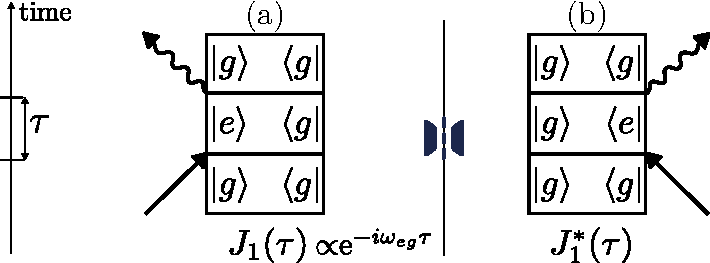
\includegraphics[width=0.6\textwidth]{figures/spctr_linear_response_feynman_diagrams.pdf}
	\caption{First-order double-sided Feynman diagrams contributing to linear response. (a) Interaction on the ket (left action). (b) Interaction on the bra (right action). The commutator in~\autoref{eq:S1_def_superop_thesis} is their difference~\cite{mukamel1995principlesnonlinearoptical}.}
	\label{fig:linear_response_diagrams}
\end{figure}

\subsubsection{Frequency-Domain Susceptibility and Absorption}
The linear susceptibility is the Fourier transform of the causal response kernel \autoref{eq:R1_J1_J1*},
\begin{equation*}
	\chi^{(1)}(\omega)
	= \int_{-\infty}^{\infty}\!\mathrm{d}\tau\,R^{(1)}(\tau)\,
	\mathrm{e}^{\mathrm{i}\omega\tau}
	= \int_0^{\infty}\!\mathrm{d}\tau\,R^{(1)}(\tau)\,
	\mathrm{e}^{\mathrm{i}\omega\tau}.
\end{equation*}
With this, \autoref{eq:P1_convolution_thesis} becomes in frequency space
\begin{equation*}
	\boldsymbol{P}^{(1)}(\omega) = \chi^{(1)}(\omega)\!\cdot\!\boldsymbol{E}(\omega).
\end{equation*}
Conventional line shapes can be connected to the pathway functions $J_1(\tau)$ and $J_1^*(\tau)$ defined in~\autoref{eq:J1_definitions}, by approximating the coherence pathway through the Green function, $J_1(\tau)\propto G_{eg}(\tau)$.
This yields
\begin{equation*}
	\int_0^{\infty}\!\mathrm{d}\tau\,
	G_{eg}(\tau)\,\mathrm{e}^{\mathrm{i}\omega\tau}
	= \frac{1}{\Gamma_{eg}+\mathrm{i}(\omega_{eg}-\omega)},
\end{equation*}
and therefore the familiar complex Lorentzian susceptibility
\begin{equation*}
	\chi^{(1)}(\omega)
	\propto d^2
	\frac{1}{\Gamma_{eg} - \mathrm{i}(\omega-\omega_{eg})}.
\end{equation*}
Its imaginary part gives the absorptive line shape centred at $\omega_{eg}$ with half-width $\Gamma_{eg}$, and the absorption coefficient satisfies $\alpha(\omega)\propto \operatorname{Im}\chi^{(1)}(\omega)$.
For multiple excited states $e_i$, the total absorption is a sum over allowed $g\to e_i$ transitions.

\subsection{Nonlinear Response}
\label{sec:third_order_response}
Even-order susceptibilities vanish in centrosymmetric media, so the lowest-order nonlinear response relevant here is third order~\cite{boyd2008chapter6nonlinear,mukamel1995principlesnonlinearoptical}.
The central $\chi^{(3)}$ process for this thesis is four-wave mixing (FWM)~\cite{boyd2008chapter6nonlinear}, in which three incident fields generate a signal field.
The resulting photon-echo and free-induction-decay contributions form the basis of 2D spectroscopy.

\subsubsection{Third-Order Response Function \texorpdfstring{$R^{(3)}$}{R(3)}}
Inserting $n=3$ into~\autoref{eq:app_Pn_convolution_scalar} and~\autoref{eq:app_Sn_def_scalar} gives
\begin{equation}
\label{eq:P3_convolution_thesis}
\boldsymbol{P}^{(3)}(t)
= \int_{0}^{\infty}\!\mathrm{d}\tau_3\int_{0}^{\infty}\!\mathrm{d}\tau_2\int_{0}^{\infty}\!\mathrm{d}\tau_1\,
R^{(3)}(\tau_3,\tau_2,\tau_1)\,
E(t-\tau_3)\,E(t-\tau_3-\tau_2)\,E(t-\tau_3-\tau_2-\tau_1),
\end{equation}
with response function
\begin{equation}
\label{eq:S3_def_thesis}
R^{(3)}(\tau_3,\tau_2,\tau_1)
= (\mathrm{i})^3\,\mathrm{Tr}\Bigl\{\hat{\boldsymbol{\mu}}\,\mathcal{U}_0(\tau_3)\,\mathcal{V}\,\mathcal{U}_0(\tau_2)\,\mathcal{V}\,\mathcal{U}_0(\tau_1)\,\mathcal{V}[\hat{\rho}_{\mathrm{eq}}]\Bigr\}.
\end{equation}
This third-order response contains the multi-time correlations central to the present thesis.
Reading the operator product in~\autoref{eq:S3_def_thesis} from right to left corresponds to the causal sequence: start from $\hat{\rho}_{\mathrm{eq}}$, apply a dipole interaction, evolve freely, apply another interaction, and so on, followed by the dipole readout at time $t$.
In a three-pulse experiment one writes $E(t)=E_1(t)+E_2(t)+E_3(t)$; inserting this into~\autoref{eq:P3_convolution_thesis} generates many terms, and the experimentally relevant contribution (e.g.\ rephasing) is selected by phase matching or phase cycling.
The material kernel responsible for that selection is precisely~\autoref{eq:S3_def_thesis}~\cite{hammzanni2011conceptsmethods2d}.

\subsubsection{Two-Level System and Pathway Expansion}
\label{sec:two_level_third_order_pathways}
To see concretely how higher-order expressions expand, consider again the two-level system from \autoref{sec:two_level_system_linear_response}.
After the first interaction $\mathcal{V}$, $\hat{\rho}_{\mathrm{S}}$ is a linear combination of the coherences $\ket{e}\!\bra{g}$ and $\ket{g}\!\bra{e}$, followed by free evolution during $\tau_1$, which imprints phase factors $G_{eg}(\tau_1)$ and $G_{eg}^*(\tau_1)$ (see~\autoref{eq:Green_function_two_level,eq:S1_commutator_expanded}).
A second light--matter interaction converts these coherences into populations,
\begin{equation*}
    \mathcal{V}[\ket{e}\!\bra{g}] \approx \ket{g}\!\bra{g} - \ket{e}\!\bra{e},
    \qquad
    \mathcal{V}[\ket{g}\!\bra{e}] \approx \ket{e}\!\bra{e} - \ket{g}\!\bra{g}.
\end{equation*}
During $\tau_2$, the density operator is (in this simple model) a linear combination of populations.
The third commutator converts populations back into coherences, which evolve during $\tau_3$.
Finally, left multiplication by $\hat{m}$ and the trace yield the measurable polarisation.

Writing the nested commutator~\autoref{eq:S3_def_thesis} explicitly,
\begin{equation*}
	R^{(3)}(\tau_3,\tau_2,\tau_1)
	=(-i)\,
	\mathrm{Tr}\Big\{\hat{\mu}_{\mathrm{I}}(\tau_{1}+\tau_{2}+\tau_{3})\,[\hat{\mu}_{\mathrm{I}}(\tau_{1}+\tau_{2}),[\hat{\mu}_{\mathrm{I}}(\tau_1),[\hat{\mu}_{\mathrm{I}}(0),\hat{\rho}_{\mathrm{eq}}]]]\Big\},
\end{equation*}
one obtains the $2^3=8$ operator products
\begin{align}
	\label{eq:R3_commutator_expansion_R1R4_S4}
	R^{(3)}(\tau_3,\tau_2,\tau_1) & = \mathrm{Tr}\big\{\hat{\mu}_{\mathrm{I}}(\tau_{1}+\tau_{2}+\tau_{3})\,\hat{\mu}_{\mathrm{I}}(\tau_{1}+\tau_{2})\,\hat{\mu}_{\mathrm{I}}(\tau_1)\,\hat{\mu}_{\mathrm{I}}(0)\,\hat{\rho}_{\mathrm{eq}}\big\}
	\quad\Rightarrow\quad R_4
	\\
	\label{eq:R3_commutator_expansion_R1R4_S1star}
	                              & -\,\mathrm{Tr}\big\{\hat{\mu}_{\mathrm{I}}(\tau_{1}+\tau_{2}+\tau_{3})\,\hat{\mu}_{\mathrm{I}}(\tau_{1}+\tau_{2})\,\hat{\mu}_{\mathrm{I}}(\tau_1)\,\hat{\rho}_{\mathrm{eq}}\,\hat{\mu}_{\mathrm{I}}(0)\big\}
	\quad\Rightarrow\quad R_1^{*}
	\\
	\label{eq:R3_commutator_expansion_R1R4_S2star}
	                              & -\,\mathrm{Tr}\big\{\hat{\mu}_{\mathrm{I}}(\tau_{1}+\tau_{2}+\tau_{3})\,\hat{\mu}_{\mathrm{I}}(\tau_{1}+\tau_{2})\,\hat{\mu}_{\mathrm{I}}(0)\,\hat{\rho}_{\mathrm{eq}}\,\hat{\mu}_{\mathrm{I}}(\tau_1)\big\}
	\quad\Rightarrow\quad R_2^{*}
	\\
	\label{eq:R3_commutator_expansion_R1R4_S3}
	                              & +\,\mathrm{Tr}\big\{\hat{\mu}_{\mathrm{I}}(\tau_{1}+\tau_{2}+\tau_{3})\,\hat{\mu}_{\mathrm{I}}(\tau_{1}+\tau_{2})\,\hat{\rho}_{\mathrm{eq}}\,\hat{\mu}_{\mathrm{I}}(0)\,\hat{\mu}_{\mathrm{I}}(\tau_1)\big\}
	\quad\Rightarrow\quad R_3
	\\
	\label{eq:R3_commutator_expansion_R1R4_S3star}
	                              & -\,\mathrm{Tr}\big\{\hat{\mu}_{\mathrm{I}}(\tau_{1}+\tau_{2}+\tau_{3})\,\hat{\mu}_{\mathrm{I}}(\tau_1)\,\hat{\mu}_{\mathrm{I}}(0)\,\hat{\rho}_{\mathrm{eq}}\,\hat{\mu}_{\mathrm{I}}(\tau_{1}+\tau_{2})\big\}
	\quad\Rightarrow\quad R_3^{*}
	\\
	\label{eq:R3_commutator_expansion_R1R4_S2}
	                              & +\,\mathrm{Tr}\big\{\hat{\mu}_{\mathrm{I}}(\tau_{1}+\tau_{2}+\tau_{3})\,\hat{\mu}_{\mathrm{I}}(\tau_1)\,\hat{\rho}_{\mathrm{eq}}\,\hat{\mu}_{\mathrm{I}}(0)\,\hat{\mu}_{\mathrm{I}}(\tau_{1}+\tau_{2})\big\}
	\quad\Rightarrow\quad R_2
	\\
	\label{eq:R3_commutator_expansion_R1R4_S1}
	                              & +\,\mathrm{Tr}\big\{\hat{\mu}_{\mathrm{I}}(\tau_{1}+\tau_{2}+\tau_{3})\,\hat{\mu}_{\mathrm{I}}(0)\,\hat{\rho}_{\mathrm{eq}}\,\hat{\mu}_{\mathrm{I}}(\tau_1)\,\hat{\mu}_{\mathrm{I}}(\tau_{1}+\tau_{2})\big\}
	\quad\Rightarrow\quad R_1
	\\
	\label{eq:R3_commutator_expansion_R1R4_S4star}
	                              & -\,\mathrm{Tr}\big\{\hat{\mu}_{\mathrm{I}}(\tau_{1}+\tau_{2}+\tau_{3})\,\hat{\rho}_{\mathrm{eq}}\,\hat{\mu}_{\mathrm{I}}(0)\,\hat{\mu}_{\mathrm{I}}(\tau_1)\,\hat{\mu}_{\mathrm{I}}(\tau_{1}+\tau_{2})\big\}
	\quad\Rightarrow\quad R_4^{*}.
\end{align}
Along the same lines as in linear response, the terms labelled $R_\alpha^{*}$ are the complex conjugates of $R_\alpha$ for Hermitian $\hat{\mu}$ and a real equilibrium state.
In typical 2DES calculations (RWA) one therefore groups the response as
\begin{equation}
	R^{(3)}(\tau_3,\tau_2,\tau_1)
	= (-i) \sum_{\alpha=1}^{4}\Big[ R_{\alpha}(\tau_3,\tau_2,\tau_1) - R_{\alpha}^{*}(\tau_3,\tau_2,\tau_1) \Big].
	\label{eq:S3_commutator_expansion_R1R4_S1_S4star}
\end{equation}

The four pathway classes from~\autoref{eq:S3_commutator_expansion_R1R4_S1_S4star} are shown in~\autoref{fig:dsfd_R1_R4}.
\begin{figure}[htbp]
	\centering
	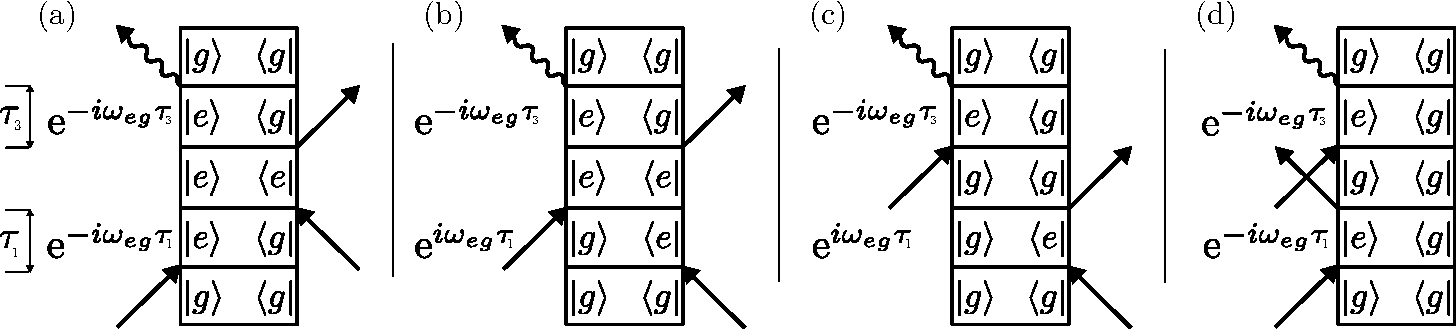
\includegraphics[width=1.0\textwidth]{figures/spctr_third_response_feynman_diagrams.pdf}
	\caption{Double-sided Feynman diagrams for the four third-order pathway classes $R_1$--$R_4$ in~\crefrange{eq:R3_commutator_expansion_R1R4_S4}{eq:R3_commutator_expansion_R1R4_S4star}.
	Each diagonal arrow indicates a field interaction acting on the ket (left branch) or bra (right branch) of the density matrix.
	The complex-conjugate pathways $R_\alpha^{*}$ correspond to exchanging ket and bra actions as in~\autoref{fig:linear_response_diagrams}.}
	\label{fig:dsfd_R1_R4}
\end{figure}
For interpretation, the eight third-order pathways are regrouped into physical classes~\cite{mukamel1995principlesnonlinearoptical, cho2009twodimensionalopticalspectroscopy}:
\begin{itemize}
	\item \textbf{Ground-state bleach (GSB).} During the waiting time $\tau_2$ the system resides in the ground-state population $\ket{g}\!\bra{g}$. The third interaction probes the depleted ground-state absorption.
	\item \textbf{Stimulated emission (SE).} During $\tau_2$ the system resides in the excited-state population $\ket{e}\!\bra{e}$. The third interaction stimulates emission back to the ground state.
	\item \textbf{Excited-state absorption (ESA).} During $\tau_2$ the system is in $\ket{e}\!\bra{e}$, but the third interaction promotes it to a higher-lying state $\ket{f}$. ESA is absent in the simple two-level as it requires an additional  electronic state (see~\autoref{sec:multilevel_generalization_thesis}).
\end{itemize}
GSB and SE contribute with the same sign, whereas ESA enters with the opposite sign.

\paragraph{Phase factors of the individual pathways.}
Reading off the coherence Green function (cf.~\autoref{sec:two_level_third_order_pathways}) for each Feynman diagram yields
\begin{align}
    \exp\bigl[-\mathrm{i}\omega_{eg}\,& f_n(\tau_3,\tau_1)\bigr],\\
    R_1 \text{\&} R_4:\quad & f_{1/4}(\tau_3,\tau_1) = \tau_3 + \tau_1,\\
    R_2 \text{\&} R_3:\quad & f_{2/3}(\tau_3,\tau_1) = \tau_3 - \tau_1,
    \label{eq:pathway_phase_functions}
\end{align}
Populations during the second period $\tau_2$ carry no rapid oscillation.
However, during $\tau_2$, population relaxation modifies the third-order pathways.
For the two-level system, the dissipative channel can be described phenomenologically by the Lindblad jump operator $\hat{L}=\sqrt{\gamma_{ge}}\,\ket{g}\!\bra{e}$, which implements $\ket{e}\to\ket{g}$ at rate $\gamma_{ge}$.
The resulting equations of motion for the density-matrix elements are
\begin{align}
	\dot{\rho}_{ee} &= -\gamma_{ge}\,\rho_{ee}, &
	\dot{\rho}_{gg} &= +\gamma_{ge}\,\rho_{ee}, &
	\dot{\rho}_{eg} &= -(\gamma_{ge}/2 + \gamma_\varphi)\,\rho_{eg},
\end{align}
where $\gamma_\varphi$ accounts for additional pure dephasing.
Solving these gives the population propagators
\begin{equation}
	U_{ee,ee}(\tau_2) = \mathrm{e}^{-\gamma_{ge}\tau_2},\qquad
	U_{gg,ee}(\tau_2) = 1-\mathrm{e}^{-\gamma_{ge}\tau_2},\qquad
	U_{gg,gg}(\tau_2) = 1,
	\label{eq:population_propagators_two_level_thesis}
\end{equation}
and the total dephasing rate of the optical coherence is $\Gamma_{eg}=\gamma_{ge}/2+\gamma_{\varphi}$, with $T_1=1/\gamma_{ge}$ and $T_2=1/\Gamma_{eg}$.

Consequently, every pathway through $\rho_{ee}$ during $\tau_2$ splits into two contributions: one remaining in $ee$ (multiplied by $U_{ee,ee}$) and one relaxed to $gg$ (multiplied by $U_{gg,ee}$).

For the two-level system, the third-order response $R^{(3)}$ thus contains contributions from GSB and SE only.
In practice, $R^{(3)}$ is computed by summing the available pathways---contributions automatically generated by the Liouvillian propagator.
Having established the third-order response function $R^{(3)}(\tau_3,\tau_2,\tau_1)$ in~\autoref{sec:third_order_response} as the material kernel encoding the microscopic dynamics, the experimental realisation is now specified: a sequence of three controllable laser pulses.
This enables the isolation of different subsets of pathways via phase matching or phase cycling, in particular separating rephasing and nonrephasing signals.

%------------------------------------------------------------------------------
% 4. Three-Pulse Experiments and Phase Matching
%------------------------------------------------------------------------------
\section{Three-Pulse Experiments and Phase Matching}
\label{sec:three_pulse_geometry}
In a three-pulse experiment, the measured third-order signal is obtained by driving the system with a sequence of fields and reading out the radiated polarisation.
For finite-duration pulses with partial overlap, the separation into strictly time-ordered interactions is approximate and the signal becomes a convolution of the material response with the pulse envelopes, which modifies pathway weights and phases~\cite{hammzanni2011conceptsmethods2d, doetal2017simplifiedexpressionsthat}.
In this thesis these effects are captured directly by the nonperturbative simulations.

\subsection{Electric Fields}
\label{subsec:electric_fields}
The applied field is written as a sum of three pulses with carrier wavevectors $\boldsymbol{k}_1,\boldsymbol{k}_2,\boldsymbol{k}_3$ and carrier frequency $\omega_L$,
\begin{equation}
	\boldsymbol{E}(\boldsymbol{r},t)
	=
	\sum_{j=1}^{3}
	\Big[
	\boldsymbol{E}_j(t-t_j)\,e^{\mathrm{i}(\boldsymbol{k}_j\cdot\boldsymbol{r}-\omega_{L} t + \phi_j)}
	+ \text{c.c.}
	\Big],
	\label{eq:E_three_pulses_space}
\end{equation}
where $t_j$ denotes the arrival time of pulse $j$, $\phi_j$ its carrier phase, and $\boldsymbol{E}_j(t)$ a complex envelope.
In the rotating-wave approximation, the field is decomposed into positive- and negative-frequency parts,
\begin{equation}
    \boldsymbol{E}(\boldsymbol{r},t) = \boldsymbol{E}^{(+)}(\boldsymbol{r},t) + \boldsymbol{E}^{(-)}(\boldsymbol{r},t),\qquad
    \boldsymbol{E}^{(-)} = \bigl[\boldsymbol{E}^{(+)}\bigr]^*,
    \label{eq:E_plusminus}
\end{equation}
with analytic part
\begin{equation*}
	\boldsymbol{E}^{(+)}(\boldsymbol{r},t)
	=
	\sum_{j=1}^{3}
	\boldsymbol{E}_j(t-t_j)\,
	e^{\mathrm{i}(\boldsymbol{k}_j\cdot\boldsymbol{r}-\omega_{L} t + \phi_j)}.
\end{equation*}
Under the RWA, only the near-resonant cross terms $\hat{\boldsymbol{\mu}}^{(+)}\!\cdot\!\boldsymbol{E}^{(-)}$ and $\hat{\boldsymbol{\mu}}^{(-)}\!\cdot\!\boldsymbol{E}^{(+)}$ are retained~\cite{mukamel1995principlesnonlinearoptical,boyd2008chapter6nonlinear}.
Consequently, contributions to the nonlinear polarisation acquire phase factors $\pm\boldsymbol{k}_j$ and $\pm\phi_j$.
These are exploited for pathway selection by phase matching and phase cycling (see~\autoref{sec:phase_cycling}).
An optional Bloch-sphere intuition for carrier-phase kicks and pulse area is provided in~\autoref{app:phase_kick_intuition}; the main text here continues with the phase-matching formulation used in the simulations.

\subsection{Wavevector Phase-Matching Condition}
\label{subsec:phase_matching_condition}
In nonlinear wave mixing, the signal is emitted into directions that satisfy energy and momentum conservation, $\Delta\boldsymbol{k}\approx 0$.
In a plane-wave picture, momentum conservation implies that the signal wavevector $\boldsymbol{k}_{\mathrm{S}}$ is a signed sum of the input wavevectors,
\begin{equation}
	\boldsymbol{k}_{\mathrm{S}} = \pm\boldsymbol{k}_1 \pm \boldsymbol{k}_2 \pm \boldsymbol{k}_3.
	\label{eq:four_wave_mixing}
\end{equation}
This is the \emph{phase-matching condition}.
The signs track whether the interaction involves $\boldsymbol{E}^{(+)}$ or $\boldsymbol{E}^{(-)}$ (see~\autoref{eq:E_plusminus}).
Equivalently, in Liouville space they track whether the interaction acts on the ket or bra branch of the density matrix: absorption-like interactions contribute $+\boldsymbol{k}_j$, while emission-like/complex-conjugate interactions contribute $-\boldsymbol{k}_j$.

Different sign choices correspond to different phase-matched signal directions and hence to different subsets of Liouville-space pathways.
In noncollinear geometries these directions can be spatially separated.
The experimental geometry considered here is shown in~\autoref{fig:fwm_box_car_setup}; it defines $\boldsymbol{k}_1$, $\boldsymbol{k}_2$, $\boldsymbol{k}_3$ and the signal direction $\boldsymbol{k}_{\mathrm{S}}$ used below.

\begin{figure}[htbp]
	\centering
	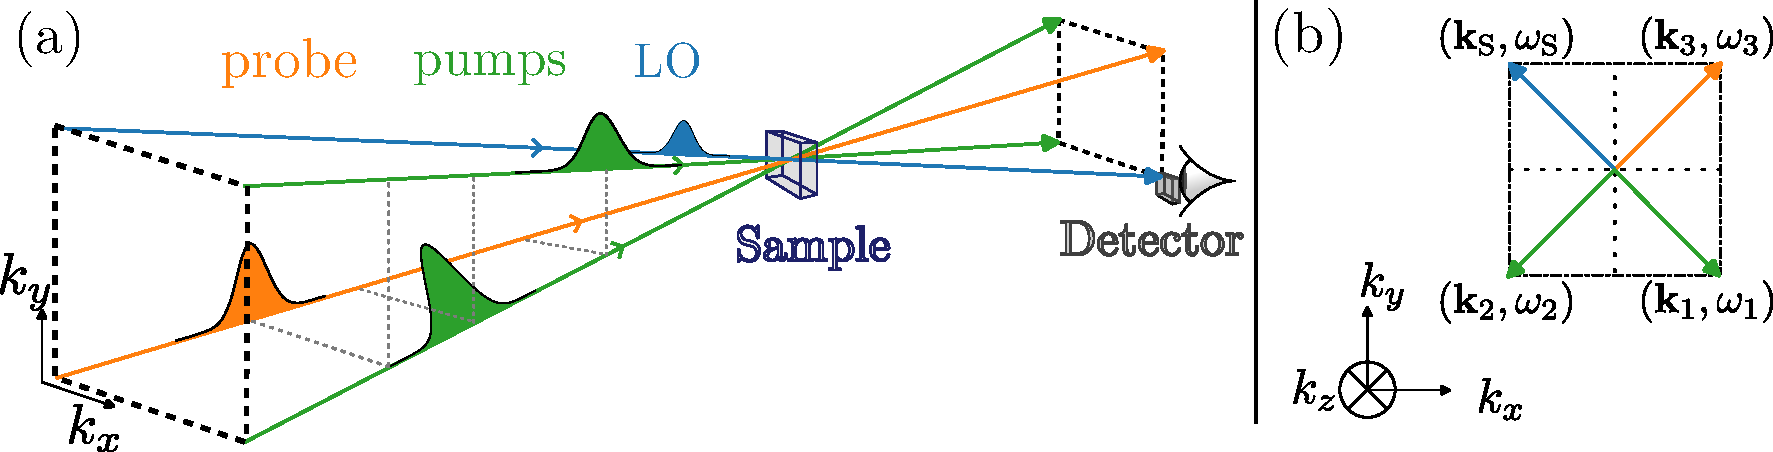
\includegraphics[width=0.9\textwidth]{figures/spctr_fwm_boxcar_schematic.pdf}
	\caption{Noncollinear BOXCARS geometry. (a) Beam arrangement in the $k_x$--$k_y$ plane with three input beams (green/orange) and the signal direction $\boldsymbol{k}_{\mathrm{S}}$ (blue); shaded envelopes indicate relative pulse timing. (b) Wavevector diagram showing the relation between $\boldsymbol{k}_1$, $\boldsymbol{k}_2$, $\boldsymbol{k}_3$, and $\boldsymbol{k}_{\mathrm{S}}$, with the corresponding frequency labels $\omega_j$ and $\omega_{\mathrm{S}}$.}
	\label{fig:fwm_box_car_setup}
\end{figure}

\subsection{Rephasing and Nonrephasing Phase-Matching Conditions}
\label{subsec:rephasing_nonrephasing}
Inserting the three-pulse field~\autoref{eq:E_three_pulses_space} into the third-order convolution~\autoref{eq:P3_convolution_thesis} and allowing only RWA-resonant terms, the third-order polarisation decomposes into components labelled by a sign triple $(l,m,n)$ with $l,m,n\in\{-1,+1\}$,
\begin{equation}
	\boldsymbol{P}^{(3)}(\boldsymbol{r},t)
	=
	\sum_{l,m,n}
	e^{\mathrm{i}(\boldsymbol{k}_{\mathrm{S}}\cdot\boldsymbol{r} - \omega_{L} t + \Phi_{lmn})}\,
	\boldsymbol{P}^{(3)}_{l,m,n}(t),
	\qquad
	\boldsymbol{k}_{\mathrm{S}} = l\boldsymbol{k}_1+m\boldsymbol{k}_2+n\boldsymbol{k}_3,\quad
	\Phi_{lmn} = l\phi_1+m\phi_2+n\phi_3.
	\label{eq:P3_lmn}
\end{equation}
The triple $(l,m,n)$ labels the sign choices for each of the three interactions; as noted above, these determine the ket/bra assignment for each interaction step via the phase-matching condition.
Only combinations satisfying the macroscopic phase-matching condition contribute efficiently in an extended sample~\cite{boyd2008chapter6nonlinear}.

The two third-order directions of interest for 2DES are
\begin{align}
	\boldsymbol{k}_{\mathrm{R}}    & = -\boldsymbol{k}_1 + \boldsymbol{k}_2 + \boldsymbol{k}_3, \label{eq:kR_def} \\
	\boldsymbol{k}_{\mathrm{NR}} & = +\boldsymbol{k}_1 - \boldsymbol{k}_2 + \boldsymbol{k}_3,
	\label{eq:kNR_def}
\end{align}
usually identified as \emph{rephasing} (R) and \emph{nonrephasing} (NR) directions, respectively~\cite{mukamel1995principlesnonlinearoptical, cho2009twodimensionalopticalspectroscopy, freschetal2023twodimensionalelectronicspectroscopy}.

Besides the RWA, a useful limiting case is the impulsive limit of well separated pulses, where the interaction times are strictly ordered and pulse overlap can be neglected~\cite{cho2009twodimensionalopticalspectroscopy,mukamel1995principlesnonlinearoptical}.
Then the sign patterns in~\crefrange{eq:kR_def}{eq:kNR_def} can be read directly as a sequence of ket- and bra-branch interactions (see~\autoref{app:sec:phase_kick_pulse_area_intuition}).

For perfectly ordered interactions, pulses 1 and 3 determine whether the coherence phase evolves with opposite signs or with the same sign during $\tau_1$ and $\tau_3$.
Opposite signs produce the rephasing contribution; equal signs produce the nonrephasing contribution.

For the rephasing signal, the sign reversal acts like a photon echo and refocuses static disorder in an inhomogeneously broadened ensemble~\cite{jonas2003twodimensionalfemtosecondspectroscopy, cho2009twodimensionalopticalspectroscopy, freschetal2023twodimensionalelectronicspectroscopy}.
The nonrephasing signal does not refocus static disorder. However it gives a free-induction--decay response and is therefore directly sensitive to homogeneous linewidths~\cite{jonas2003twodimensionalfemtosecondspectroscopy}.
Consistently, from~\autoref{eq:pathway_phase_functions}, $R_2$ and $R_3$ carry $\exp[-\mathrm{i}\omega_{eg}(\tau_3-\tau_1)]$ (rephasing), whereas $R_1$ and $R_4$ carry $\exp[-\mathrm{i}\omega_{eg}(\tau_3+\tau_1)]$ (nonrephasing).

As a note, other third-order pathways like \textit{double-quantum coherence} can be accessed by the phase matching condition $\boldsymbol{k}_{\mathrm{S}}=+\boldsymbol{k}_1+\boldsymbol{k}_2-\boldsymbol{k}_3$.
They are not required for the aims of this thesis.
See Ref.~\cite{caietal2024extractingdoublequantumcoherence} for a broader overview.

%------------------------------------------------------------------------------
% 5. Phase Cycling in Collinear Geometry
%------------------------------------------------------------------------------
\section{Phase Cycling and Selection of Pathways}
\label{sec:phase_cycling}
In a collinear geometry, different signal wavevector components $\boldsymbol{k}_{\mathrm S}$ cannot be spatially separated.%
\footnote{In numerical simulations this limitation is even more direct: spatial propagation and beam geometry are typically not modelled, so $\boldsymbol{k}$-selection cannot be implemented at the level of the fields.}
Instead, pathway selection is achieved by \emph{phase cycling}: one repeats the measurement for different carrier-phase settings $\phi_j$ and isolates the desired contribution by a discrete Fourier projection with respect to $(\phi_1,\phi_2,\phi_3)$~\cite{mukamel1995principlesnonlinearoptical, greenetal2024vibrationalcoherenceshalfbroadband}.
This works because each Liouville-space pathway acquires a characteristic phase factor determined by the sequence of light--matter interactions.

The pulse sequence and delay definitions used throughout this work are shown in~\autoref{fig:fwm_phase_cycling_setup}.

\begin{figure}[htbp]
	\centering
	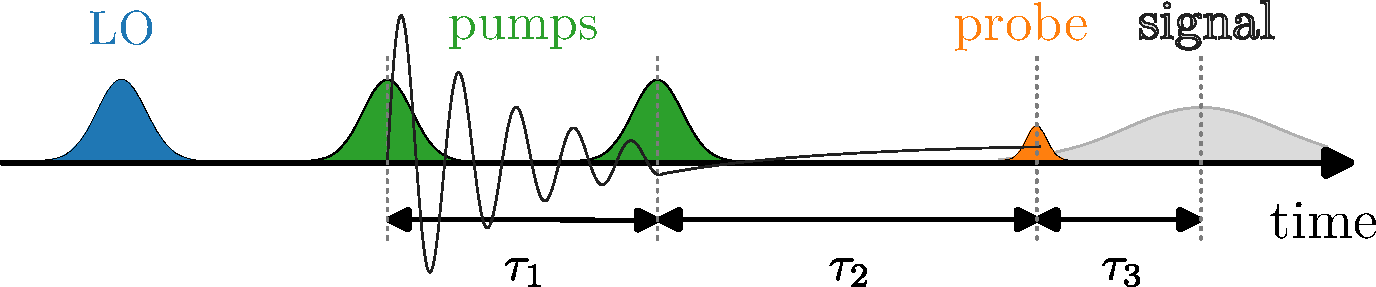
\includegraphics[width=0.85\textwidth]{figures/spctr_fwm_collinear_schematic.pdf}
	\caption{Collinear pulse sequence used for phase cycling. The local oscillator (LO, see~\autoref{sec:detection_schemes}), two pump pulses, the probe pulse, and the emitted signal are shown schematically in time. The three inter-pulse delays are labelled $\tau_1$, $\tau_2$, and $\tau_3$, with the corresponding time variables $t_{\mathrm{coh}}$, $t_{\mathrm{wait}}$, $t_{\mathrm{det}}$ indicated below.}
	\label{fig:fwm_phase_cycling_setup}
\end{figure}

The third-order polarisation is $2\pi$-periodic in each $\phi_j$ and can be expanded as a Fourier series,
\begin{equation*}
	P^{(3)}(t;\phi_1,\phi_2,\phi_3)
	=
	\sum_{l,m,n} e^{\mathrm{i}(l\phi_1+m\phi_2+n\phi_3)}\,P^{(3)}_{l,m,n}(t),
\end{equation*}
where $P^{(3)}_{l,m,n}(t)$ collects all third-order contributions carrying the phase combination $(l,m,n)$.
In particular, the rephasing and nonrephasing components correspond to
\begin{align}
	\text{rephasing:}\quad (l,m,n)    & = (-1,+1,+1),
	\label{eq:phase_rephasing}                        \\
	\text{nonrephasing:}\quad (l,m,n) & = (+1,-1,+1).
	\label{eq:phase_nonrephasing}
\end{align}
These index triples are the phase analogues of the wavevector combinations~\cref{eq:kR_def,eq:kNR_def}~\cite{mukamel1995principlesnonlinearoptical, cho2009twodimensionalopticalspectroscopy, greenetal2024vibrationalcoherenceshalfbroadband}.

In practice, one evaluates $P^{(3)}$ on a finite phase grid, typically
$\phi_j \in \{0,2\pi/N_\phi,\dots,2\pi(N_\phi-1)/N_\phi\}$ for each $j$ (often $N_\phi=4$, i.e.\ steps of $\pi/2$), which is sufficient to separate the third-order components relevant for rephasing and nonrephasing 2D spectra. The desired component is then obtained by discrete Fourier projection,
\begin{equation}
	P^{(3)}_{l,m,n}(t)
	\simeq
	\frac{1}{N_\phi^3}
	\sum_{\phi_1,\phi_2,\phi_3}
	e^{-\mathrm{i}(l\phi_1+m\phi_2+n\phi_3)}\,
	P^{(3)}(t;\phi_1,\phi_2,\phi_3).
	\label{eq:discrete_phase_cycling}
\end{equation}
In the continuous limit this becomes the inverse Fourier transform
\begin{equation}
	P^{(3)}_{l,m,n}(t)
	=
	\frac{1}{(2\pi)^3}
	\int_{0}^{2\pi}\!\!\int_{0}^{2\pi}\!\!\int_{0}^{2\pi}
	d\phi_1\,d\phi_2\,d\phi_3\;
	e^{-\mathrm{i}(l\phi_1+m\phi_2+n\phi_3)}\,
	P^{(3)}(t;\phi_1,\phi_2,\phi_3).
	\label{eq:continuous_phase_cycling}
\end{equation}

In the simulations used in this thesis, $P^{(3)}(t;\phi_1,\phi_2,\phi_3)$ is obtained by solving the full master equation, including the time-dependent light--matter interaction, for each phase setting $(\phi_1,\phi_2,\phi_3)$. The phase-selected third-order contribution is then extracted via~\autoref{eq:discrete_phase_cycling}, choosing $(l,m,n)$ according to~\cref{eq:phase_rephasing,eq:phase_nonrephasing}.

%------------------------------------------------------------------------------
% 6. Construction of Two-Dimensional Spectra
%------------------------------------------------------------------------------
\section{Construction of Two-Dimensional Spectra}
\label{sec:2D_construction_formal}
In a three-pulse experiment it is customary to parameterise the signal by the three time delays
\begin{equation*}
	t_{\mathrm{coh}}\equiv\tau_1,\qquad
	t_{\mathrm{wait}}\equiv\tau_2,\qquad
	t_{\mathrm{det}}\equiv\tau_3,
\end{equation*}
with delay variables defined in~\autoref{eq:app_change_of_variables} and used in the third-order convolution~\autoref{eq:app_Pn_convolution_scalar}.
The quantities $t_{\mathrm{coh}}$, $t_{\mathrm{wait}}$, and $t_{\mathrm{det}}$ are referred to as coherence time, waiting time, and detection time, respectively.

Scanning the waiting time $t_{\mathrm{wait}}$ probes population dynamics and spectral diffusion during the population interval between the second and third interactions~\cite{cho2009twodimensionalopticalspectroscopy, mukamel1995principlesnonlinearoptical}.

The phase-cycled complex signal field $E_{\mathrm{R/NR}}(t_{\mathrm{coh}},t_{\mathrm{wait}},t_{\mathrm{det}})$ is the object from which 2D spectra are constructed.
The Maxwell-side propagation and phase-matching assumptions underpinning $E_{\mathrm{S}}\propto P^{(3)}$ are derived in~\autoref{app:2dfts_maxwell}.
Together with the third-order material response from~\autoref{eq:P3_convolution_thesis,eq:S3_def_thesis}, this gives the central chain used throughout the thesis,
\begin{equation}
\label{eq:signal_chain_R3}
R^{(3)}\;\Longrightarrow\;P^{(3)}\;\Longrightarrow\;E_{\mathrm{S}}\;\Longrightarrow\;\tilde{E}_{\mathrm{S}}.
\end{equation}
To make explicit how the recorded quantity connects to this chain, the next subsection discusses the detection step.

\subsection{Detection: From Polarisation to Signal Field}
\label{sec:detection_schemes}
Detectors measure intensities.
In 2DES, the outgoing field is typically spectrally dispersed and recorded as a function of detection frequency $\omega_{\mathrm{det}}$.
Formally, the recorded signal is proportional to the detected intensity integrated over the detector response time,
\begin{equation}
	\tilde{E}_{\mathrm{S}}(\omega_{\mathrm{det}}) \propto \int I_{\mathrm{det}}(\omega_{\mathrm{det}},t)\,\mathrm{d}t.
	\label{eq:signal_intensity}
\end{equation}
Two common schemes differ in sensitivity and in whether phase information is retained: homodyne and heterodyne detection~\cite{abramaviciusetal2009coherentmultidimensionaloptical}.

\paragraph{Homodyne (self-heterodyne) detection.}
In \emph{homodyne} detection one records the intensity of the signal field itself,
\begin{equation}
	I_{\mathrm{HOD}}(\omega_{\mathrm{det}}) \propto \big|E_{\mathrm{S}}(\omega_{\mathrm{det}})\big|^2.
\end{equation}
This scales quadratically with the signal field (and thus with the underlying polarisation), mixes different nonlinear orders, and does not directly retain the signal phase.
Many linear experiments can be viewed as a special ``self-heterodyne'' limit where the weak generated field interferes with a strong transmitted reference field that is automatically present.

\paragraph{Heterodyne detection (explicit LO).}
In background-free four-wave-mixing geometries the signal is emitted into a distinct phase-matched direction, so no strong reference beam co-propagates with it.
One therefore introduces an explicit \emph{local oscillator} (LO) field $E_{\mathrm{LO}}$ that overlaps with the signal on the detector.
Writing the spectrally resolved total field as
\begin{equation}
	E_{\mathrm{tot}}(\omega_{\mathrm{det}}) = E_{\mathrm{LO}}(\omega_{\mathrm{det}}) + E_{\mathrm{S}}(\omega_{\mathrm{det}}),
	\label{eq:heterodyne_total_field_freq}
\end{equation}
the measured spectral intensity is
\begin{equation}
	I_{\mathrm{HET}}(\omega_{\mathrm{det}})
	\propto
	\big|E_{\mathrm{tot}}(\omega_{\mathrm{det}})\big|^2
	=
	|E_{\mathrm{LO}}(\omega_{\mathrm{det}})|^2
	+ |E_{\mathrm{S}}(\omega_{\mathrm{det}})|^2
	+ 2\,\Re\big[E_{\mathrm{LO}}^*(\omega_{\mathrm{det}})E_{\mathrm{S}}(\omega_{\mathrm{det}})\big].
	\label{eq:heterodyne_intensity_expanded_freq}
\end{equation}
For $|E_{\mathrm{S}}|\ll|E_{\mathrm{LO}}|$ the $|E_{\mathrm{S}}|^2$ term can be neglected, and the LO background $|E_{\mathrm{LO}}|^2$ can be measured and subtracted.
It is convenient to define a normalised heterodyne signal,
\begin{equation}
	\tilde{E}_{\mathrm{HET}}(\omega_{\mathrm{det}})
	\equiv
	\frac{I_{\mathrm{HET}}(\omega_{\mathrm{det}})-|E_{\mathrm{LO}}(\omega_{\mathrm{det}})|^2}{|E_{\mathrm{LO}}(\omega_{\mathrm{det}})|^2}
	\approx 2\,\Re\left[\frac{E_{\mathrm{LO}}^*(\omega_{\mathrm{det}})E_{\mathrm{S}}(\omega_{\mathrm{det}})}{|E_{\mathrm{LO}}(\omega_{\mathrm{det}})|^2}\right],
	\label{eq:heterodyne_signal_normalized}
\end{equation}
which makes explicit that heterodyne detection renders the measurement linear in the signal field.

Combining this with the field--polarisation relation from~\autoref{app:2dfts_maxwell} and the third-order polarisation from~\autoref{eq:P3_convolution_thesis,eq:S3_def_thesis} yields the proportionality used in this thesis,
\begin{equation}
\label{eq:heterodyne_chain_R3}
\tilde{E}_{\mathrm{HET}}\propto \Re\!\left[E_{\mathrm{LO}}^{*}E_{\mathrm{S}}\right]
\propto \Re\!\left[E_{\mathrm{LO}}^{*}P^{(3)}\right]
\propto \Re\!\left[E_{\mathrm{LO}}^{*}\,(R^{(3)}\ast E_1\ast E_2\ast E_3)\right].
\end{equation}
Thus, once the phase-matched/phase-cycled third-order component is isolated (\autoref{subsec:phase_matching_condition,sec:phase_cycling}), the detected heterodyne signal reports the third-order response convolved with the applied pulse sequence.

\paragraph{Phase sensitivity and phasing.}
Writing the LO as $E_{\mathrm{LO}}(\omega_{\mathrm{det}})=A(\omega_{\mathrm{det}})e^{\mathrm{i}\phi_{\mathrm{LO}}(\omega_{\mathrm{det}})}$ shows that the recorded cross term depends on the (in general unknown) LO spectral phase,
\begin{equation}
	\tilde{E}_{\mathrm{HET}}(\omega_{\mathrm{det}})
	\propto \Re\Big\{e^{-\mathrm{i}\phi_{\mathrm{LO}}(\omega_{\mathrm{det}})}\,E_{\mathrm{S}}(\omega_{\mathrm{det}})\Big\}.
	\label{eq:heterodyne_phase_sensitive}
\end{equation}
If $\phi_{\mathrm{LO}}(\omega_{\mathrm{det}})$ is not controlled or calibrated, absorptive and dispersive contributions are mixed.
Operationally, one reconstructs a complex signal (e.g.\ by spectral interferometry) and then fixes the remaining overall phase by a standard \emph{phasing} procedure (often via a pump--probe projection)~\cite{hybletal1998twodimensionalelectronicspectroscopy}.
After this calibration, the reconstructed complex $E_{\mathrm{S}}$ can be compared directly to theory.

In the numerical workflow of this thesis, the complex phase-selected signal is obtained directly from phase cycling (\autoref{eq:discrete_phase_cycling,eq:continuous_phase_cycling}), so the unknown experimental LO phase does not appear as an additional fitting parameter.

\paragraph{Remark (what is actually measured, and how to recover a complex signal).}
Even with heterodyne detection, the detector output at fixed waiting time $T$ and detection frequency is a \emph{real} function of the coherence time.
In an idealised description one may write the measured (rephasing) trace as
\begin{equation}
	\tilde{E}_{\mathrm{R}}^{(\mathrm{meas})}(\omega_{\mathrm{det}};T,t_{\mathrm{coh}})
	= \Re\big[ e^{\mathrm{i}\phi}\,\tilde{E}_{\mathrm{R}}(\omega_{\mathrm{det}};T,t_{\mathrm{coh}}) \big],
\end{equation}
where $\phi$ is an (unknown) global phase set by the relative signal/LO optical paths.
This is the global phase ambiguity discussed above in frequency-resolved form (cf.~\autoref{eq:heterodyne_phase_sensitive}).
In experiments one reconstructs a complex signal and removes this by interferometric calibration plus phasing.
In this thesis, complex $\tilde{E}_{\mathrm{R/NR}}(t_{\mathrm{coh}},T,t_{\mathrm{det}})$ is obtained directly from phase cycling in the simulations, and the extracted complex signal is then used for the Fourier-domain construction described in~\autoref{sec:2D_construction_formal}.

\textbf{Remark (positive vs.\ negative coherence time).}
In some presentations one also considers negative $t_{\mathrm{coh}}$ values, which correspond to reversing the order of pulses 1 and 2.
Then the rephasing photon-echo picture does not apply.
Instead one obtains a nonrephasing free-induction--decay-like contribution complementary to the $t_{\mathrm{coh}}>0$ rephasing branch~\cite{ginsbergetal2009twodimensionalelectronicspectroscopy}.
For each fixed waiting time $t_{\mathrm{wait}}$, the signal is a function of the two coherence times $t_{\mathrm{coh}}$ and $t_{\mathrm{det}}$,
\begin{equation*}
	E_{\mathrm{R/NR}} = E_{\mathrm{R/NR}}(t_{\mathrm{coh}},t_{\mathrm{wait}},t_{\mathrm{det}}).
\end{equation*}

\subsection{Double Fourier Transform and 2D Spectra}
After computing the time-domain polarisation (\autoref{eq:P_def_spectroscopy}) and selecting the desired phase-tagged component via phase cycling (\autoref{eq:continuous_phase_cycling}), one obtains the corresponding complex signal field $E_{\mathrm{R/NR}}(t_{\mathrm{coh}},t_{\mathrm{wait}},t_{\mathrm{det}})$ (\autoref{eq:field_polarisation_relation}).
For the nonperturbative numerical extraction, see~\autoref{eq:third_order_signal_numerical} in~\autoref{app:numerical_implementation}.
The two-dimensional spectrum is defined as the double Fourier transform of the time-domain signal with respect to $(t_{\mathrm{coh}},t_{\mathrm{det}})$ at fixed $t_{\mathrm{wait}}$.
The opposite sign in the $t_{\mathrm{coh}}$ exponent distinguishes rephasing (photon-echo) and nonrephasing branches~\cite{cho2009twodimensionalopticalspectroscopy, greenetal2024vibrationalcoherenceshalfbroadband}.

In the numerical implementation, slowly varying complex envelopes are used (the optical carrier $e^{-\mathrm{i}\omega_{L} t}$ is removed), so $\omega_{\mathrm{coh}}$ and $\omega_{\mathrm{det}}$ represent Fourier variables of these envelopes.

For the rephasing signal,
\begin{equation*}
	\tilde{E}_{\mathrm{R}}(\omega_{\mathrm{coh}},t_{\mathrm{wait}},\omega_{\mathrm{det}})
	=
	\int_{0}^{\infty}\!\mathrm{d}t_{\mathrm{det}}
	\int_{0}^{\infty}\!\mathrm{d}t_{\mathrm{coh}}\;
	e^{+\mathrm{i}\omega_{\mathrm{coh}} t_{\mathrm{coh}}}\,e^{-\mathrm{i}\omega_{\mathrm{det}} t_{\mathrm{det}}}\,
	E_{\mathrm{R}}(t_{\mathrm{coh}},t_{\mathrm{wait}},t_{\mathrm{det}}),
\end{equation*}
while for the nonrephasing signal,
\begin{equation*}
	\tilde{E}_{\mathrm{NR}}(\omega_{\mathrm{coh}},t_{\mathrm{wait}},\omega_{\mathrm{det}})
	=
	\int_{0}^{\infty}\!\mathrm{d}t_{\mathrm{det}}
	\int_{0}^{\infty}\!\mathrm{d}t_{\mathrm{coh}}\;
	e^{-\mathrm{i}\omega_{\mathrm{coh}} t_{\mathrm{coh}}}\,e^{-\mathrm{i}\omega_{\mathrm{det}} t_{\mathrm{det}}}\,
	E_{\mathrm{NR}}(t_{\mathrm{coh}},t_{\mathrm{wait}},t_{\mathrm{det}}).
\end{equation*}
In numerical implementations, finite integration limits (discrete time grids) are used and discrete Fourier transforms are applied with appropriate windowing.
On uniform grids these are evaluated efficiently via (shifted) fast Fourier transforms~\cite{cho2009twodimensionalopticalspectroscopy, greenetal2024vibrationalcoherenceshalfbroadband}.

The absorptive 2D spectrum is obtained as the real part of the sum
\begin{equation*}
	\tilde{E}_{\mathrm{abs}}(\omega_{\mathrm{coh}},t_{\mathrm{wait}},\omega_{\mathrm{det}})
	=
	\Re\Big\{ \tilde{E}_{\mathrm{R}}(\omega_{\mathrm{coh}},t_{\mathrm{wait}},\omega_{\mathrm{det}}) + \tilde{E}_{\mathrm{NR}}(\omega_{\mathrm{coh}},t_{\mathrm{wait}},\omega_{\mathrm{det}}) \Big\}.
\end{equation*}
This combination removes dispersive distortions that appear when considering $|\tilde{E}_{\mathrm{R}}|$ or $|\tilde{E}_{\mathrm{NR}}|$ alone and yields peak shapes directly comparable with experimental absorptive 2D spectra~\cite{jonas2003twodimensionalfemtosecondspectroscopy, fullerogilvie2015experimentalimplementationstwodimensional}.
The construction outlined in this chapter---from the master equation through phase-cycled polarisations to the absorptive 2D spectrum---forms the computational backbone of the numerical results presented in the following chapters.
